\subsection{Automatic Format Inference}
\label{ssec:format-inference}

When a network problem, compromised machine or malfunctioning application
has been discovered, tracing the problem or attack to
prevent a recurrence is imperative.  This forensic analysis involves
human-guided study of multiple data sources such as log files and
other audit trails.  These data sources are great stores of
information, but they come in many varied and complex forms. They can
contain errors, either unintentional or malicious, and they can be
very, very large.  

To perform forensic analysis, analysts need to quickly understand a
variety of data sources and to ask specific questions about their
contents.  The variety, volume, and complexity of the data mean that
analysts need computational tools to support their analyses and to aid
in information extraction.  However, since every system is different
and the variety of data is so extensive, it is impossible to build
proactively all the specific tools one might need.

In the case of an attack, network forensic analysis should be done in
real-time, perhaps even while an attack is still underway. Not only
does this timeliness increase the chance of discovering the attacker
directly, it also provides the opportunity of identifying and
isolating compromised machines so that the attack cannot spread
further.  Of course, even in the case where an attack or problem is not
deemed urgent, a system adminstrator's time is always valuable --
improvements in administrator efficiency will be translated into 
improvements in their employer's bottom line.

Thus forensic analysts face a twofold problem: (1) they must be able
to ask questions of a wide array of data sources, impossible to
predict in advance, and (2) they must do so highly efficiently.  If
analysts faced only problem (1), they might take their time building
custom tools to query each individual data source from scratch, 
a task that might involve parsing, query support, and visualization 
components.  If analysts faced only problem (2) for a single data source 
known well in advance, they might take the initiative to develop a 
single, standard tool.  Our challenge is to solve both (1) and (2) 
simultaneously: to provide a platform for rapid generation of 
parsing, querying and visualization components for new and evolving
application data sources.

Although PADS descriptions can make managing ad hoc data much easier,
the problem of producing the description in the first place
remains. Writing such descriptions can be tedious and time consuming,
often requiring iteration. First, analysts write a description of as
much of the data as they understand. From this description, they
generate and run analysis tools to find any unknown parts of the
data. They then study those parts and refine the description
accordingly. They repeat this process until all the data either
conforms to the description or constitutes an error in the data rather
than an error in the description.  While the web server log we displayed
earlier may seem easy enough to describe by hand, it is amongst the
simplest examples that we could choose -- application logs may be much
more involved, requiring two-, three- or five-fold more complex descriptions.  
Moreover, the complexity of the situation grows tremendously in a realistic
setting where one must deal with logs of huge size (millions of lines long)
or large archives of logs of many different kinds. 
Having a tool to help produce such descriptions and to generate
data transformation and analysis tools automatically would speed up
forensic analysis and investigation efforts enormously.

\subsubsection*{Format Inference and Tool Generation Architecture}

\begin{figure}
\begin{center}
\centerline{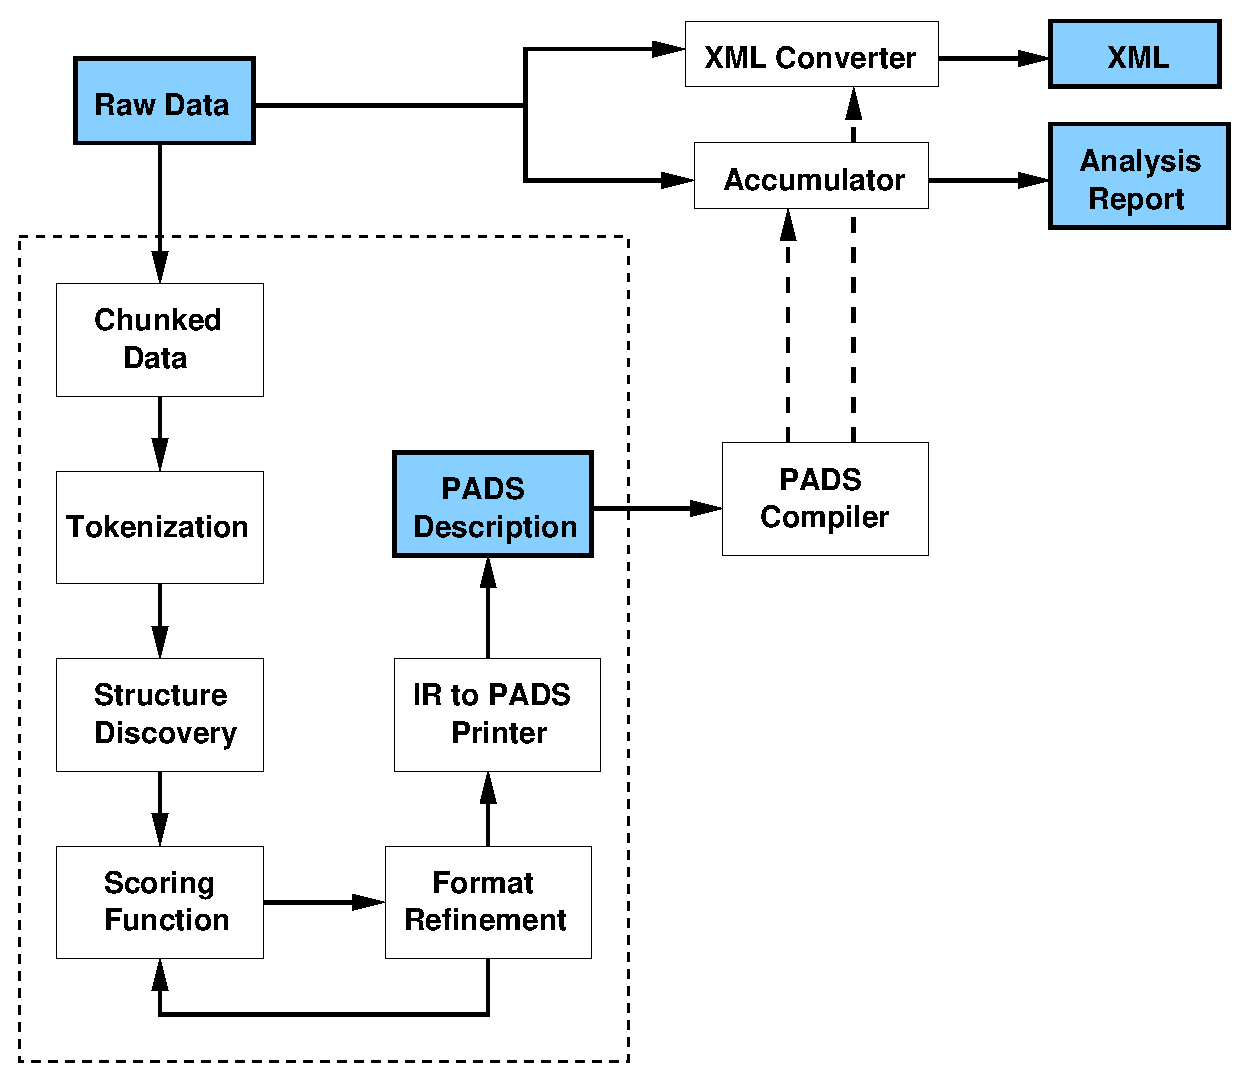
\psfig{file=format-inference-engine.eps,height=2.5in}}
\end{center}
\caption{Modular Architecture of a Format Inference and Tool Generation Engine}
\label{fig:format-inference-engine}
\end{figure}

In preparation for this proposal, we have begun to build a tool for
automatic format inference and data analysis tool generation.  In the
course of building this prototype we have defined a promising, modular 
architecture for solving the problem and performed some preliminary
experiments.  Our experiments have revealed the fact that our proposal
is indeed feasible yet many important challenges must be overcome
to turn our prototype into a robust, precise and viable system.

The overall architecture for the system is presented in
Figure~\ref{fig:format-inference-engine}.  As the diagram shows, the
system takes raw data (sets of systems or application logs) as an
input, pushes the raw data through the inference engine and generates
a \pads{} description.  This description is then automatically fed
through the current \pads{} compiler to produce several simple
data-processing tools including a tool that will read in the data and
translate it to \xml{} as well as a tool (listed in the diagram
as ``the accumulator'')
that will read in the data and output a simple statistical overview
of the data including the distribution of values in each data field and
the number of errors that it finds.

The heart of the system is a highly modular, multi-phase inference 
engine.  We have already begun work on each phase, but also have
many important research questions to answer about each part.
These phases include:

\begin{itemize}
\item {\bf Chunking:}  The first step in the inference process
is to break data into pieces, with the goal that each piece will have
a similar repetitive structure.  Currently, a user can
specify by hand that the data is either chunked line-by-line or file-by-file.
In the future we hope to develop techniques to handle several other
chunking strategies including paragraph-by-paragraph chunking or
directory-by-directory chunking of data sets.  We will develop heuristics
to guess the correct chunking structure when it is unspecified.

\item {\bf Tokenization:}  
The contents of every chunk of data must be divided up
into {\em tokens} such as numbers, words, punctuation, dates, times, 
ip addresses, phone numbers, etc.  Our current prototype includes built-in
support for a small number of basic tokens.  Our experiments indicate
effective tokenization is an extremely important element of the design, yet
astonishingly hard to achieve due ambiguities that arise in token definitions.
In particular, the {\em local} tokenization techniques we are currently using
seem insufficient for disamiguation in general and we are eager to investigate 
techniques that use more {\em global} information to achieve more precise
and useable tokenization.

\item {\bf Structure Discovery:}
After tokenization, the structure discovery phase produces a
candidate format for the data being analyzed.  This candidate is
produced through a recursive divide-and-conquer algorithm that uses
various heuristics to split the data into pieces, analyze the subpieces,
generate formats for subpieces and then combine generated formats to
create an overall description.  This divide-and-conquer algorithm
works well in many cases but occasionally fails, producing \pads{} 
descriptions that do not parse all of the data in the test set.
The reason for this failure is that not all \pads{} features (which
include features from context-free grammars as well as a certain kind
of {\em context-sensitive} grammar) will 
{\em compose} properly with one another.\footnote{Technically, we require
that if $D_1$ and $D_2$ are \pads{} descriptions, then the language of their
concatenation $L(D_1 . D_2)$ must be equivalent to the concatenation
of their languages $L(D_1) . L(D_2)$ and likewise for union and Kleene
closure.  \pads{}, which, for performance reasons, and to handle important
{\em non-context free} features such as dependencies and back references, 
is defined similarly
to the PEGS family of grammars does not have this critical property, 
which is the norm for context-free grammars.}  Hence, in order to overcome
this central problem and develop a robust inference engine, we must
investigate how to redesign several of the core elements of 
the \pads{} language, an interesting theoretical and implementation
challenge.

\item {\bf Scoring Function and Format Rewriting:}
The format generated by the structure discovery is only a rough ``guess''
at the structure of a format.  It is often unnecessarily complicated
in some places and too limited in others.  In order to improve the 
quality of the guess, we score the format and then search for ways
to optimize it using a collection of format rewriting rules.  The
score is based upon the information-theoretic principles embodied in
the Minimum Description Length Principle (MDL)~\cite{mdl}.  In our
experience to date, this format rewriting is somewhat effective --
it reduces the score of the formats initially produced substantially.
However, to the human eye, much improvement can still be made.  We must
investigate the sources of the problems, develop new rewriting rules
and refine the scoring function which guides which rules to apply and
when. 
\end{itemize}

In addition to studying, evaluating, and improving each of the phases
of the inference engine mentioned above, we will engage in two additional
tasks with regards to this element of the grant:

\begin{itemize}
\item {\bf Scaling to large data sets:}
\item {\bf Wholistic repository inference:}
\end{itemize}

\paragraph*{Summary of Format Inference:}  
We have developed a prototype
format inference engine for system log files.  This prototype demonstrates
our ability and the viability of our approach.  However, all phases of
our prototype engine (chunking, tokenization, structure discovery,
scoring and rewriting) must be improved in order to deliver a reliable and
effective automatic tool generation engine.  Moreover, we must develop
completely new algorithms in order to scale our current system up to 
be able to handle application log files of realistic size and complexity.
Finally, we must develop new techniques to extend the scope of our engine
so that it can analyze and uncover the structure
of entire repositories full of log files.